\documentclass[review]{elsarticle}

\usepackage{lineno,hyperref}
\modulolinenumbers[5]

\usepackage[top=2.54cm, bottom=2.54cm, left=2.54cm, right=2.54cm]{geometry}
\usepackage{amsmath}
\usepackage{graphicx}
\usepackage{subfig}
\renewcommand{\thesubfigure}{\Alph{subfigure}}% uppercase subfloat numbering
\graphicspath{{../figures/}}


\journal{Journal of Theoretical Biology}

%%%%%%%%%%%%%%%%%%%%%%%
%% Elsevier bibliography styles
%%%%%%%%%%%%%%%%%%%%%%%
%% To change the style, put a % in front of the second line of the current style and
%% remove the % from the second line of the style you would like to use.
%%%%%%%%%%%%%%%%%%%%%%%

%% Numbered
%\bibliographystyle{model1-num-names}

%% Numbered without titles
%\bibliographystyle{model1a-num-names}

%% Harvard
%\bibliographystyle{model2-names.bst}\biboptions{authoryear}

%% `Elsevier LaTeX' style
\bibliographystyle{elsarticle-num}
%%%%%%%%%%%%%%%%%%%%%%%

\begin{document}

\begin{frontmatter}

\title{Neural crest cell migration with continuous states}

%% Group authors per affiliation:
\author{Linus J. Schumacher\fnref{myfootnote}}
\address{MCR Centre for Regenerative Medicine, University of Edinburgh}
\ead{Linus.Schumacher@ed.ac.uk}


\begin{abstract}
...
\end{abstract}

\begin{keyword}
collective behaviour \sep cell migration \sep neural crest \sep developmental biology
\MSC[2010] 92C15
\end{keyword}

\end{frontmatter}

\linenumbers

\section{Introduction}
\paragraph{Neural crest cell migration is a popular example of collective cell behaviour in development ... It works like so and is important because ...  and cancer \cite{Kulesa2006,Bailey2012,McLennan2017} Multiple groups have addressed the problem with mathematical modelling \cite{Simpson2007,Landman2011,Carmona-Fontaine2011,Wynn2012,Wynn2013,McLennan2012,McLennan2015,Mort2016,Zhang2018,Merchant2018}}

\paragraph{Previous work has shown that chick cranial neural crest cell migration can be described with discrete leader-follower states that alternatively undergo chemotaxis or contact-guidance \cite{McLennan2012,McLennan2015}, and switch between the two on a non-zero timescale based on VEGF signals \cite{McLennan2015b} This has been confirmed in a number of ways, including gene expression \cite{McLennan2015}, and recently scRNAseq \cite{Morrison2017} which provide an opportunity to investigate heterogeneity in a less biased way}

\paragraph{What has not been investigated is whether cell states need be discrete, or can be continuous. Such questions are now just within reach of being able to address \cite{Wagner2016}. this is relevant in light of ongoing debate in the literature \cite{Schumacher2016a,Richardson2016,Genuth2018}, and the difficulty of inferring heterogeneity, e.g. from tracking data \cite{Schumacher2017} Here we revisit the scRNAseq data \cite{Morrison2017} using a variety of analysis tools ... to show that a continuum of cell states is not ruled out by the data. We then modify previous models \cite{McLennan2015,McLennan2015b} to assess what effect a continuum of cell guidance behaviours has on the collective migration in this particular setting. we find that ...}

\section{Results}
reflective boundary conditions \cite{Kulesa2010,Szabo2016a}
\paragraph{choice model}
The role of stochasticity has also been investigated in other aspects of neural crest migration, such as colonization of the gut \cite{Binder2015,Smadbeck2015,Zhang2018} and pigmentation patterning \cite{Mort2016}

\paragraph{combination model}

\paragraph{Fig1: single cell gene expression}
\begin{figure}
\centering
{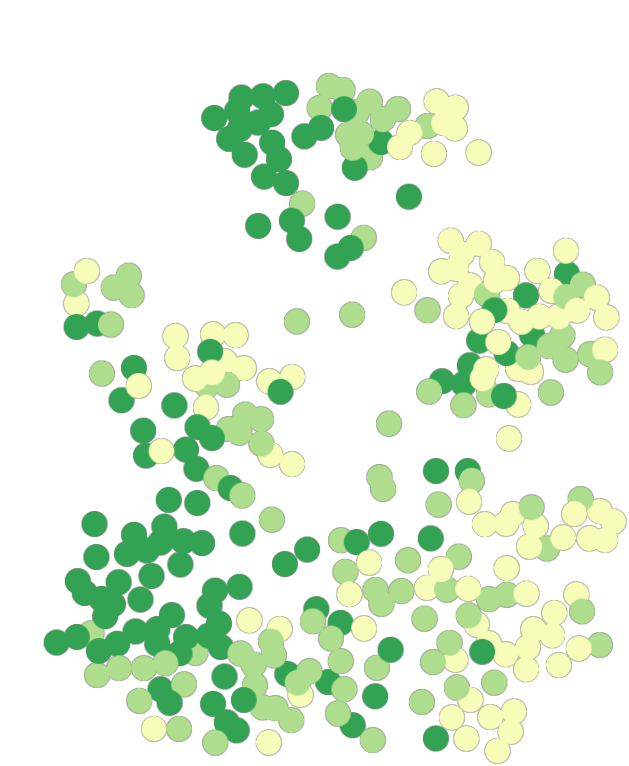
\includegraphics[scale=0.25]{Neural_Crest_NC_59PCs_HH1315}}
\caption{Visualisation of a continuum of neural crest cell states. Single-cell RNAseq data \cite{Morrison2017} from chick cranial neural crest (Hamburger-Hamilton stages 13 and 15, 310 cell sin total) taken from distinct locations in the migratory stream (trail: dark green, lead: light green, invasive front: pale yellow) were projected onto two dimensions for visualisation using a force-based embedding method \cite{Weinreb2018}. Only the top 59 principal components (out of 14299 genes measured, 12909 after preprocessing) were retained prior to embedding, based on random-matrix analysis \cite{Aparicio2018} (Fig.~\ref{figMP}).\label{figscRNAseq}}
\end{figure}

\paragraph{Fig2: modified model (a) stochastic choice (b) continuous combination} %% add some schematics
\begin{figure}
\centering
\subfloat[]{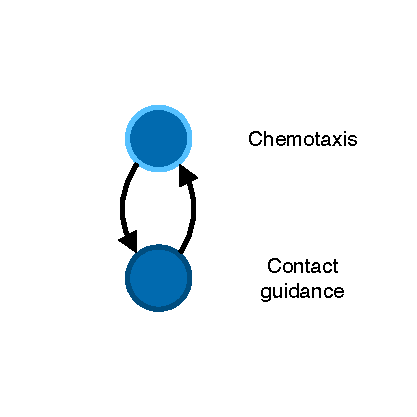
\includegraphics[]{modelSchematicControl}}
\subfloat[]{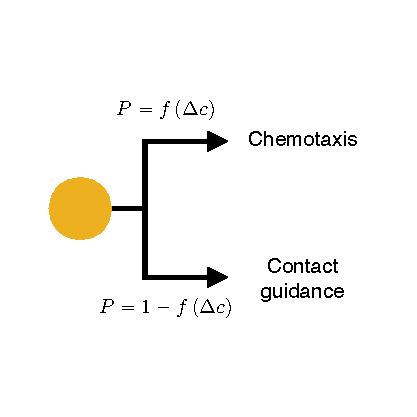
\includegraphics[]{modelSchematicChoice}}
\subfloat[]{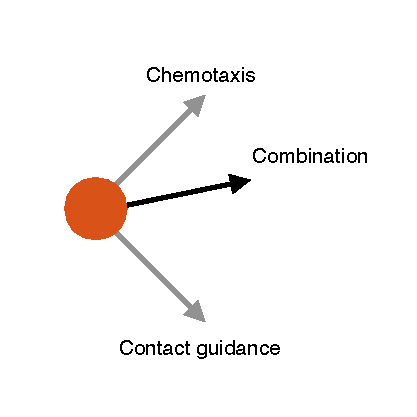
\includegraphics[]{modelSchematicCombination}}\\
\subfloat[]{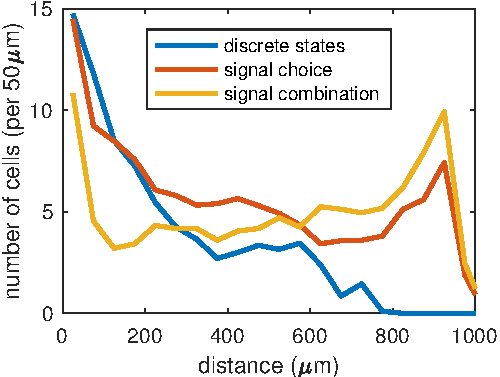
\includegraphics[]{Fig2_contStates_combination_sensAcc_10}}
\subfloat[]{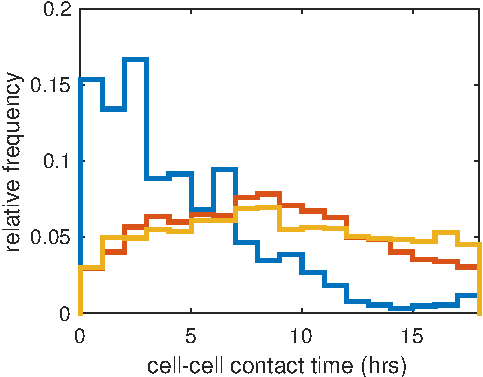
\includegraphics[]{Fig2B_contStates_combination_sensAcc_10}}
\caption{Comparison of collective cell migration models with discrete and continuous states. (A) In the previously published model \cite{McLennan2015b}, cells switch between migratory states based on the presence of a chemotactic signal and at a non-zero timescale. (B) In the signal choice model, cells choose between chemotaxis and contact guidance for their direction of movement, with a probability related to the strength of the gradient signal. In results shown here, we have used $P_\mathrm{ch}=\Delta c$ for chemotaxis and $P_\mathrm{cg}=1 - \Delta c$ for contact guidance. (C) In the signal combination model, cells combine the directional information from both chemotaxis and contact guidance, with a weighting depending on the strength of the gradient signal. Here we have used a linear weight of $\Delta c$. (D) Migration profiles of the three models after 18h of migration. (E) Durations of cell-cell contacts during migration for the three models. Line colors as in (D) \label{figNaiveModel}}
\end{figure}

\paragraph{Fig3: further model comparison}
\begin{figure}
\centering
\subfloat[]{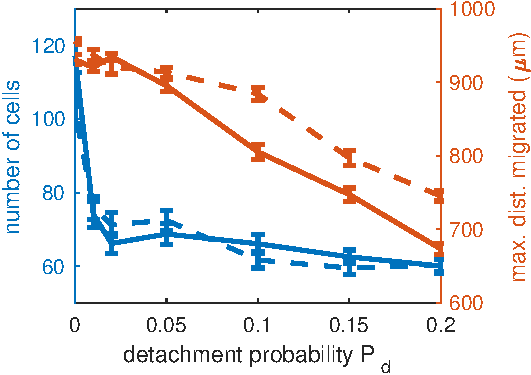
\includegraphics[]{Fig3_contStates_Psa_sensAcc_10}}\
\subfloat[]{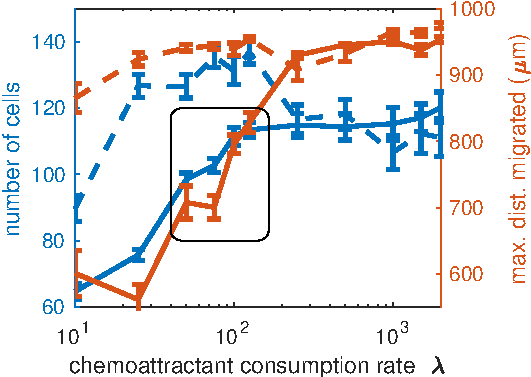
\includegraphics[]{Fig3_contStates_eat_sensAcc_10}}
\caption{Modifications to the continuous-state models can achieve experimentally realistic results. (A) Introducing a detachment probability, $P_d$, for the filopodial contacts used for contact guidance decreases the maximum distance migrated, but only at the cost of decrease total cell number for both the signal choice model (dashed lines) and the signal combination model (solid lines). (B) Reducing the chemoattractant consumption rate, $\lambda$, to the range of 40-150 (arbitrary units per hour) achieves realistic maximum distances migrated, with only a moderate reduction in cell number (highlighted by the black rectangle) for the signal combination model (solid lines), but not the signal choice model (dashed lines). Error bars show standard error of the mean.\label{figFurtherModel}}
\end{figure}

\section{Conclusions}
\paragraph{naive model with continuous states can be too good, we can make models work equally well, but need to change ..., for which we need other data? or other methods for dealing with various sources of noice in single cell data to decompose ``vectors of cellular identity'' \cite{Wagner2016}}

\paragraph{managed to fix combination model by changing chemo consumption. it is possible that this may also have worked by choosing a non-linear relationship for the weighting in combining chemotaxis and contact guidance. Further to this, one could refine the model by making the chemoconsumption proportional to leaderness, based on VEGF receptor expression.}

\paragraph{Distance migrated is not absolutely quantified experimentally, due to embryo-to-embryo variation, and lack of clearly defined start-point. Thus it is possible that the combination model describes the migration profile adequately. Also for high diffusivities, i.e. unbound VEGF, the distance migrated approached the previously observed values, as do the cell numbers (for a 2D slice approximation). Yet long-contacts in these models seem unrealistic.}

\paragraph{ One could investigate pulling \cite{Yates2018}, restraining factors \cite{McLennan2017}, do inference on parameters \cite{Ross2017}. Extension to 3D could reduce distance moved in x direction.}

\paragraph{We have unified competing views in the literature? our previous work still stands, as an approximation? This approach could be relevant beyond neural crest cell migration, such as development of the lateral line \cite{Dona2013} and asymmetry in the brain \cite{Roussigne2018} in zebrafish, \textsl{Drosophila} border cells \cite{Inaki2012}}

\section*{Acknowledgements} I would like to thank Franziska Matth\"aus for persistent suggestions.
\section*{Appendix}
\renewcommand{\thefigure}{S\arabic{figure}}
\setcounter{figure}{0}
\renewcommand{\thesection}{S}
\paragraph{Fig. S1: additional sc gene expression analysis plots}
\begin{figure}
\centering
\subfloat[]{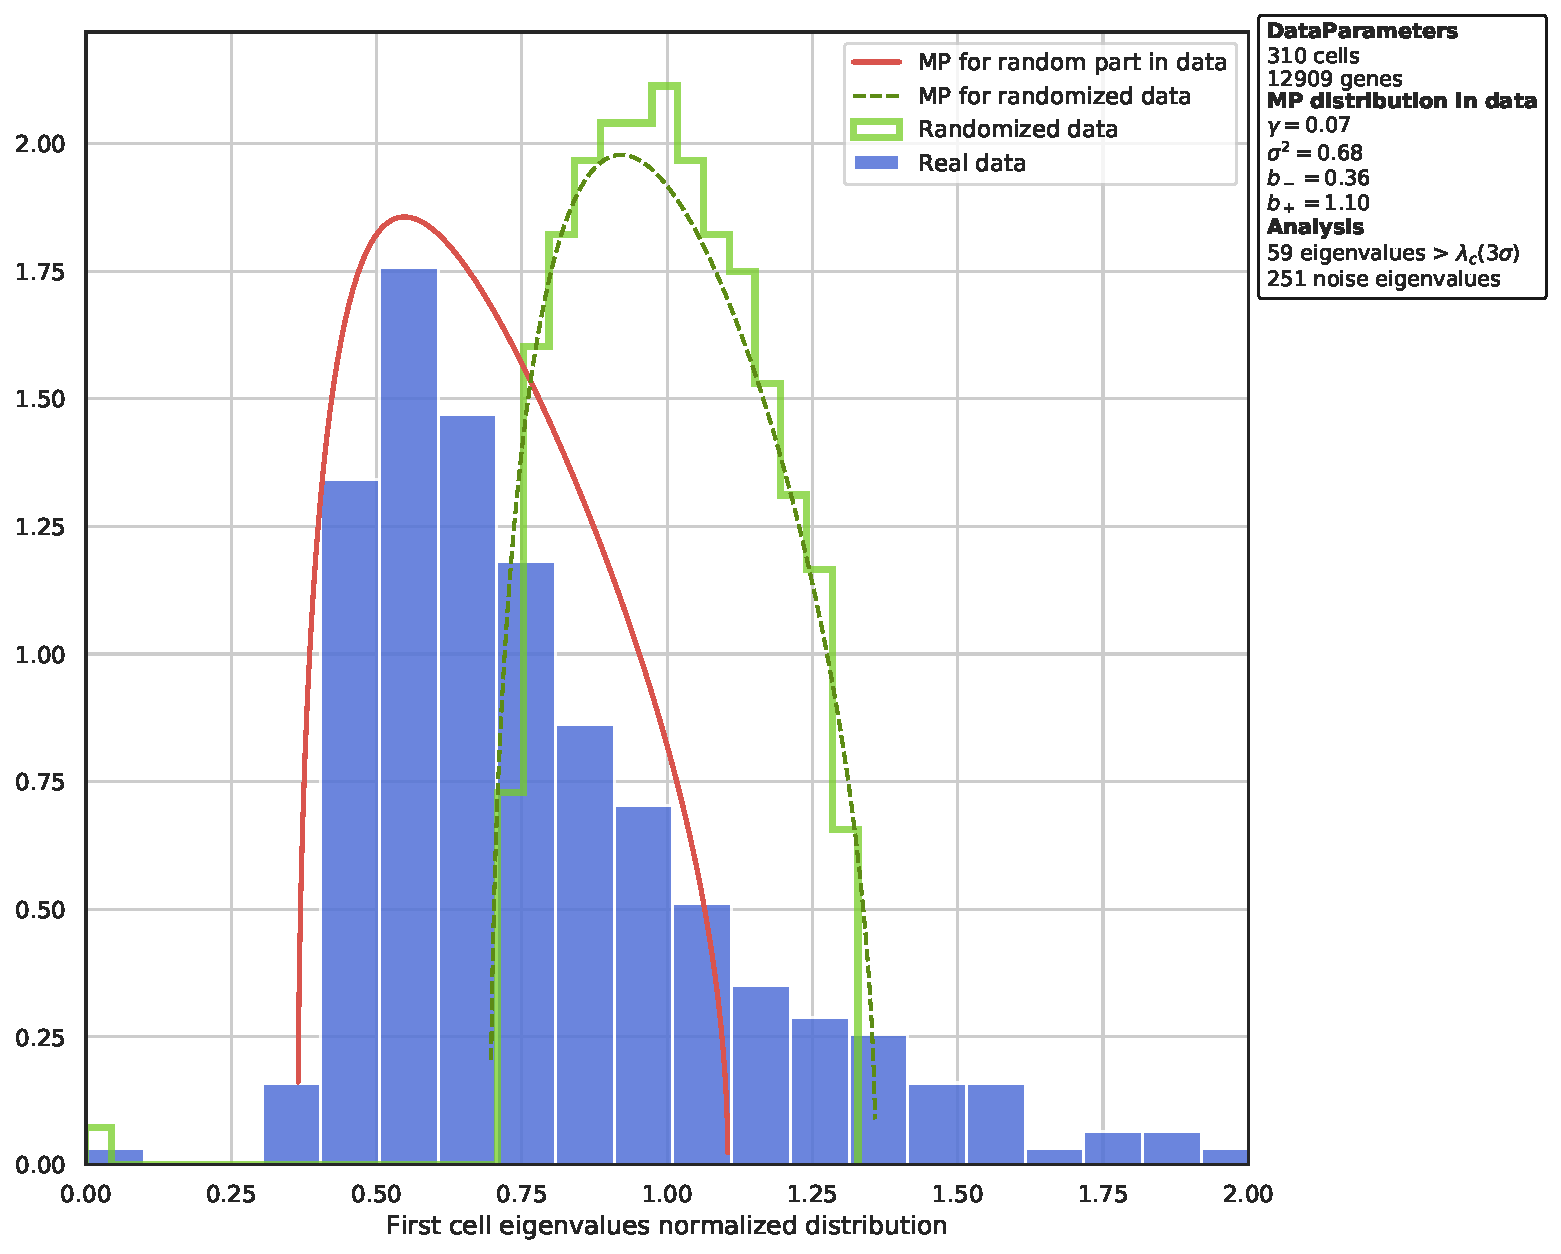
\includegraphics[scale=0.7]{mp_NC_HH1315}}
\caption{Distribution of eigenvalues of the cross-correlation matrix as calculated by the ``randomly'' software package \cite{Aparicio2018} for the single-cell RNAseq data from \cite{Morrison2018}. Bigger eigenvalues correspond to principal components that explain more variance of the data. Random matrix theory predicts that the eigenvalues of the cross-correlation matrix of a matrix independent identically distributed random variables are distributed according to the Marchenko-Pastur law. Thus, a certain amount of correlation in a data-set is to be expected under the null model of independence, here shown in red, and only principal components with large enough eigenvalues are treated as signal (here, the top 59 eigenvalues). \label{figMP}}
\end{figure}


\paragraph{Fig. S2: parameter sweeps of naive model}
\begin{figure}
\centering
\subfloat[]{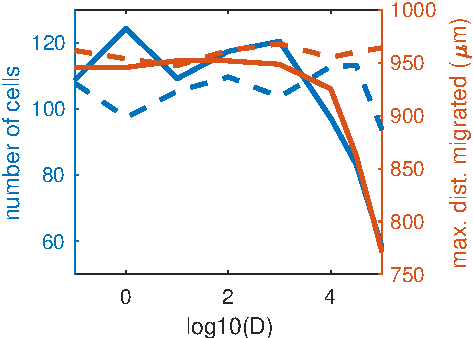
\includegraphics[]{FigS2_contStates_diffus_sensAcc_10}}\quad
\subfloat[]{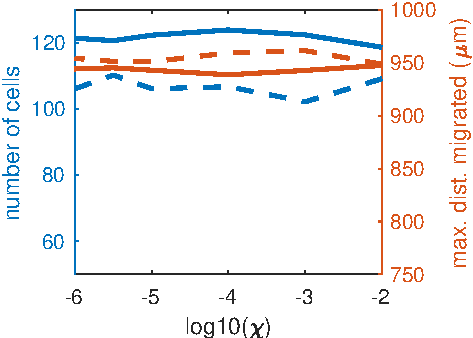
\includegraphics[]{FigS2_contStates_chi_sensAcc_10}}\\
\subfloat[]{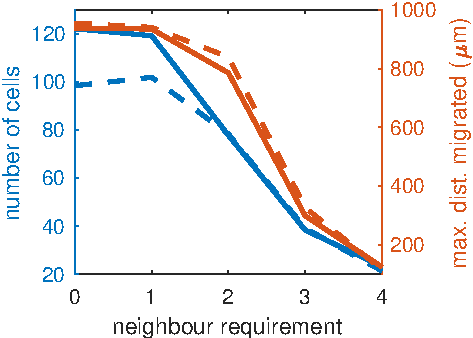
\includegraphics[]{FigS2_contStates_needNbrs_sensAcc_10}}
\caption{... \label{figNaiveModelSweeps}}
\end{figure}

\paragraph{Fig. S3: additional simulation tests, eg transplant simulations}

\section*{References}
\bibliography{references}

\end{document}